
\documentclass[12pt,a4paper,openany]{book}

%Uporabljeni paketi
\usepackage{fancyhdr}
\usepackage{graphicx}
\usepackage{color}
\usepackage{xcolor}
\usepackage[slovene]{babel}



\usepackage[utf8]{inputenc}
\usepackage[pdftex,bookmarks=true]{hyperref}

%Velikost strani - dvostransko
\oddsidemargin 1.4cm
\evensidemargin 0.35cm
\textwidth 14cm
\topmargin 0.26cm
\headheight 0.6cm
\headsep 1.5cm
\textheight 20cm

%Nastavitev glave in repa strani
\pagestyle{fancy}
\fancyhead{}
\renewcommand{\chaptermark}[1]{\markboth{\textsf{Poglavje \thechapter:\ #1}}{}}
\renewcommand{\sectionmark}[1]{\markright{\textsf{\thesection\  #1}}{}}
\fancyhead[RE]{\leftmark}
\fancyhead[LO]{\rightmark}
\fancyhead[LE,RO]{\thepage}
\fancyfoot{}
\renewcommand{\headrulewidth}{0.0pt}
\renewcommand{\footrulewidth}{0.0pt}

\newtheorem{theorem}{Izrek}[section]
\newtheorem{lemma}[theorem]{Lemma}
\newtheorem{proposition}[theorem]{Proposition}
\newtheorem{corollary}[theorem]{Corollary}

\newenvironment{proof}[1][Proof]{\begin{trivlist}
\item[\hskip \labelsep {\bfseries #1}]}{\end{trivlist}}
\newenvironment{definition}[1][Definition]{\begin{trivlist}
\item[\hskip \labelsep {\bfseries #1}]}{\end{trivlist}}
\newenvironment{example}[1][Example]{\begin{trivlist}
\item[\hskip \labelsep {\bfseries #1}]}{\end{trivlist}}
\newenvironment{remark}[1][Remark]{\begin{trivlist}
\item[\hskip \labelsep {\bfseries #1}]}{\end{trivlist}}

\newcommand{\qed}{\nobreak \ifvmode \relax \else
      \ifdim\lastskip<1.5em \hskip-\lastskip
      \hskip1.5em plus0em minus0.5em \fi \nobreak
      \vrule height0.75em width0.5em depth0.25em\fi}

%********************************************

\begin{document}

% stran 1 med uvodnimi listi
\thispagestyle{empty} 

\begin{center}
{\large 
UNIVERZA V LJUBLJANI\\
FAKULTETA ZA RAČUNALNIŠTVO IN INFORMATIKO\\
}

 
\includegraphics[scale=0.2,keepaspectratio=true]{./pictures/uni_logo.png}


\vspace{1.5cm}
{\LARGE Daniel Rižnar, Uroš Kosič}\\

\vspace{2cm}
\textsc{\textbf{\LARGE 
Umetna inteligenca 2
}}

\vspace{2cm}
{ SEMINARSKA NALOGA}\\
{ POROČILO }\\

\vspace{2cm} 
{\Large Mentor: Martin Možina}

\vfill
{\Large Ljubljana, 2011}
\end{center}

\newpage

%********************************************

\renewcommand\thepage{} 
\tableofcontents 
\renewcommand\thepage{\arabic{page}}

\thispagestyle{empty}




\setcounter{page}{1}
\pagenumbering{arabic}

\chapter*{Povzetek}

\addcontentsline{toc}{chapter}{Povzetek}
Namen dokumenta je, predstaviti naše delo, ki se je izvajalo v sklopu vaj pri predmetu
 Porazdeljene inteligentne programske tehnologije. Cilj vaj je bil implementirati znanja
 in ideje, ki smo jih pridobili pri predmetu. Implementacija je v obliki agenta, ki sodeluje
 z drugimi agenti pri igranju igre Capture The Flag (CTF). Asistent pri predmetu nam je pripravil
 simulirano okolje agenta, v katerem se igra odvija.
\\
V tem dokumentu se bomo dotaknili problemov, kot so raziskovanje prostora z več agenti, sodelovanje med agenti, 
iskanje zastave, ter razne ofenzivne in defenzivne taktike pri sami igri.
\\
Pri raziskovanju prostora je cilj, podobno kot pri raziskovanju z enim samim agentom, minimizirati skupen porabljen čas.
 V našem primeru je cil, da agenti v čim krajšem času odkrijejo zastavo. Glavni problem, ki ga je potrebno rešiti v kontekstu
 raziskovanja z večimi agenti je izbira primernih smernic za posameznega agenta, tako da istočasno raziskujejo različne predele 
prostora. Tega smo se lotili tako, da vsak agent oceni ceno poti do ciljne točke in njen prispevek. Ob vsakem morebitnem srečanju 
pa si izmenjajo informacijo o prostoru, ki so jo do tistega trenutka pridobili.\\
\\
\\
Za oblikovanje tega dokumenta je bil uporabljen sistem \LaTeX.

\vspace{1.3cm}
\noindent
{\large \bf Ključne besede:}

\vspace{0.5cm}
\noindent
Agenti, sodelovanje, CTF, raziskovanje, algoritmi, AI.



%********************************************

\chapter{Opis naloge}
RPG (role-playing game) ali igra igranja vlog je izraz za igre, v katerih igralci prevzamejo vloge namišljenih likov, postavljenih v domišljijsko okolje. Bodisi z neposrednim igranjem, bodisi z opisovanjem njihovih dejanj nato igrajo te vloge v zgodbi, ki je lahko vnaprej začrtana ali pa nastaja sproti. Uspeh ali neuspeh njihovih dejanj določa dogovorjen sistem pravil konkretne igre. Velik problem je ravnotežje različnih likov, saj se v večini primerov izkaže, da imajo nekateri liki prednost pred ostalimi in lažje zmagujejo v neposrednih dvobojih.

Posamezna RPG igra ponuja izbiro med več različnimi bojevniki, vsak ima svoje prednosti in slabosti. V tem poglavju bomo opisali konkretne značilnosti naše igre in predstavili problem.

\section{Značilnosti igre}
V igri sodelujeta dva igralca, vsak s svojim bojevnikom. Bojno polje je plošča poljubne velikosti, razdeljena na kvadratno mrežo. Bojevnika izmenično izvajate v naprej definirane akcije. Cilj igre je pokončati nasprotnika, preden on pokonča tebe. Vsak bojevnik ima na izbiro v naprej določene akcije, ki jih opisuje tabela ~\ref{table:akcijeBojevnikov}. Posamezni bojevnik je opisan z atributi, ki jih podaja ~\ref{table:atributiBojevnikov}.


\begin{table}[ht] \caption{Akcije bojevnikov}
\centering
\begin{tabular}{cp{10cm}}
\hline\hline
Akcija & Opis Akcije \\ [0.5ex]
%heading 
\hline 
Move & Akcija pomeni premik v eno izmed štirih smeri (gor, dol, levo, desno). Vsak premik zahteva določeno količino energije.\\
Pass & Akcija pomeni počitek, bojevniku se ob počivanju poveča energija.\\
Fire & Strel s primarnim orožjem. Vsak strel pomeni zmanjšanje določene količine energije in zmanjšanje življenja nasprotnika. Škoda je delno odvisna tudi od naključja.\\ [1ex]
\hline %inserts single line
\end{tabular}
\label{table:akcijeBojevnikov} % is used to refer this table in the text
\end{table}

\begin{table}[ht] \caption{Atributi bojevnikov}
\centering
\begin{tabular}{cp{10cm}}
\hline\hline
Atribut & Opis Atributa \\ [0.5ex]
%heading 
\hline 
Life & Celo število, ki podaja preostalo življenje.\\
Speed & Hitrost, ki opisuje za koliko kock se bojevnik lahko premakne ob premikih.\\
Energy & Preostala energija bojevnika, ki jo lahko porabi za izvajanje akcij.\\ [1ex]
\hline %inserts single line
\end{tabular}
\label{table:atributiBojevnikov} % is used to refer this table in the text
\end{table}

\section{Bojevniki}
Za potrebe seminarske naloge, smo se omejili le na dva bojevnika - Tank in Vojak. 
Značilnosti obeh smo določili kot v tabeli ~\ref{table:bojevniki}. 
\begin{table}[ht] \caption{Značilnosti bojevnikov}
\centering
\begin{tabular}{ccccccc}
\hline\hline
Tip & Trpežnost & Domet & Hitrost & Obnavljanje & Varčnost  & Energija \\ [0.5ex]
%heading 
\hline 
Tank & boljša & boljši & višja & slabše & boljša & višja\\
Vojak & slabša & slabši & nižja & boljše & slabša & nižja\\ [1ex]
\hline %inserts single line
\end{tabular}
\label{table:bojevniki} % is used to refer this table in the text
\end{table}


\section{Opis problema}
Znan problem v RPG igrah je ravnotežje različnih likov, ki tekmujejo med seboj. Kljub različnim lastnostim, morajo imeti bojevniki enake možnosti za zmago v igri. Naša naloga je bila poiskati konkretne vrednosti atributov za zgoraj opisana bojevnika tako, da bosta igrala čim bolj izenačeno igro. Problem smo ločili na dva dela - simulacijo igranja in optimizacijo izenačenosti bojevnikov. Za simulacijo igranja smo uporabili \textit{minimax} algoritem. Za optimizacijo smo uporabili \textit{genetske algoritme} in jih primerjali s \textit{hill climbing}-om.

\chapter{Metode dela}
V tem poglavju bomo opisali uporabljene algoritme in načine izvajanja meritev. Na koncu poglavja bomo podali nekaj implementacijskih podrobnosti.

\section{Simulacija igranja}
Za simulacijo igranja igre smo uporabili algoritem \textit{minimax}. Z njim smo poskušali doseči, da igralca igrata čim bolj optimalno igro, tj. v danem trenutku izbereta najboljšo možno potezo.

\subsection{Algoritem minimax}
Algoritem se uporablja za minimizacijo možne izgube, pri maksimizaciji možnega dobička. V naši igri igralca izmenjujeta poteze in poskušata izbrati najboljšo svojo potezo oz. maksimizirati svojo vrednost, posledično pa minimizirati nasprotnikovo. Tako glede na trenutno pozicijo identificiramo igralca MIN in MAX. Tisti ki je na potezi predstavlja igralca MAX, nasprotnik pa igralca MIN. Algoritem gradi drevo, kjer je v sodih nivojih (z začetkom v korenu) na potezi igralec MAX, na lihih pa igralec MIN. Na MAX nivojih, igralec vedno izbere stanje, ki maksimizira njegovo vrednost, na MIN nivojih pa igralec izbere stanje, ki minimizira njegovo vrednost (ker predpostavlja, da bo nasprotnik izvedel za njega najslabšo možno potezo). Naslednja poteza je tista poteza, ki jo igralec MAX izbere v korenskem vozlišču. Algoritem je predstavljen na Sliki ~\ref{fig:minimax}. Propagiranje vrednosti vozlišč poteka od spodaj navzgor, zato je potrebno te vrednosti določiti v listih. Ker je prostor preiskovanja prevelik (če bi lahko preiskali celoten prostor, bi v listih vedno imeli samo dve možnosti - zmago ali poraz), je potrebno višino drevesa omejiti, vrednost v listih pa določiti z neko hevristiko. Naša hevristika je predstavljena na ~\ref{eq:hevristika}. 

\begin{figure}[ht]
\centering

\[
  val(n) = \left\{ 
  \begin{array}{l l}
    -1000 & \quad \textrm{če je igralec MAX mrtev}\\
    +1000 & \quad \textrm{če je igralec MIN mrtev}\\
    +1.0\cdot MaxLifeRatio-1.2\cdot MinLifeRatio+ \\+0.1
 \cdot MaxEnergyRatio -0.1\cdot MinEnergyRatio & \quad \textrm{sicer}\\
  \end{array} \right.
\]
\caption[Hevristika]{Hevristika. Členi v tretjem delu funkcije predstavljajo razmerje med trenutnimi in izačetnimi vrednostmi atributov. Intuitivno, hevristika bo ocenila stanje kot dobro, če je življenje MAX igralca visoko, MIN igralca nizko, energija MAX igralca visoka in MIN igralca nizka.}
\label{eq:hevristika}
\end{figure}


\begin{figure}[ht]
 \centering
 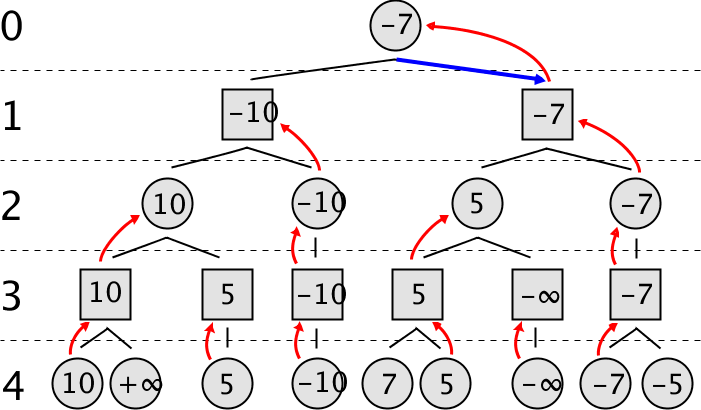
\includegraphics[width=10cm]{svg2raster.png}
 \caption[Algoritem Minimax]{Algoritem minimax: slika predstavlja delovanje algoritma minimax. Številke v vozliščih predstavljajo vrednost posameznega stanja z vidika MAX igralca. Puščice predstavljajo propagacijo vrednosti od spodaj navzgor (igralec MIN na lihih nivojih izbira minimalno vrednost, izgralec MAX na sodih nivojih izbira maksimalno vrednost).}
 \label{fig:minimax}
\end{figure}

\subsection{Problemi in prilagoditve}
V naši igri pomembno vlogo igra tudi naključje. Akcija Fire ima definirano maksimalno in minimalno škodo, ki jo zadane nasprotniku. Vsakič ko bojevnik izbere to akcijo, se vrže kocka, ki z verjetnostjo 0.5 določi stopnjo škode (ali maksimalna ali minimalna). Zaradi naključnosti, rezultati minimax algoritma ob istih vhodnih podatkih niso vedno enaki. Da bi omilili vpliv naključnosti, je potrebno igro simulirati večkrat, kar privede do povečanja časovne kompleksnosti (sicer za konstanto, a ker se ena simulacija izvaja precej časa, že ta konstanta pomeni veliko razliko). Zato smo implementirali \textit{alfabeta} rezanje, ki ob zagotavljanju enake rešitve kot navaden \textit{minimax} v večini primerov zmanjša število evaluacij listov. Na Sliki ~\ref{fig:alfabeta} je prikazan minimax algoritem z alfabeta rezanjem.
\\
\\
Z do zdaj opisanimi pravili igre se je pojavljal problem bežanja. Velikokrat se je zgodilo, da je bojevnik, ki je ugotovil da ne more zmagati, začel bežati pred drugim. Tako je igra trajala zelo dolgo ali pa se sploh ni končala. Zato smo v igro uvedli pravilo, da se bežočega bojevnika kaznuje. Pravilo smo definirali kot: če se nek bojevnik odmakne od drugega in ga v naslednji potezi nasprotnik zadane, se mu hitrost razpolovi. V primeru, da se bežoči umakne izven dosega nasprotnika, se nasprotniku moč zadetka zmanjša za $2^d$, kjer je d razdalja med bežočim in zunanjo mejo dosega akcije. Tako bežočega upočasnimo in damo nasprotniku možnost, da ga dohiti oziroma pokonča. Zdaj se bojevniki manjkrat odločajo za bežanje.


\begin{figure}[ht]
 \centering
 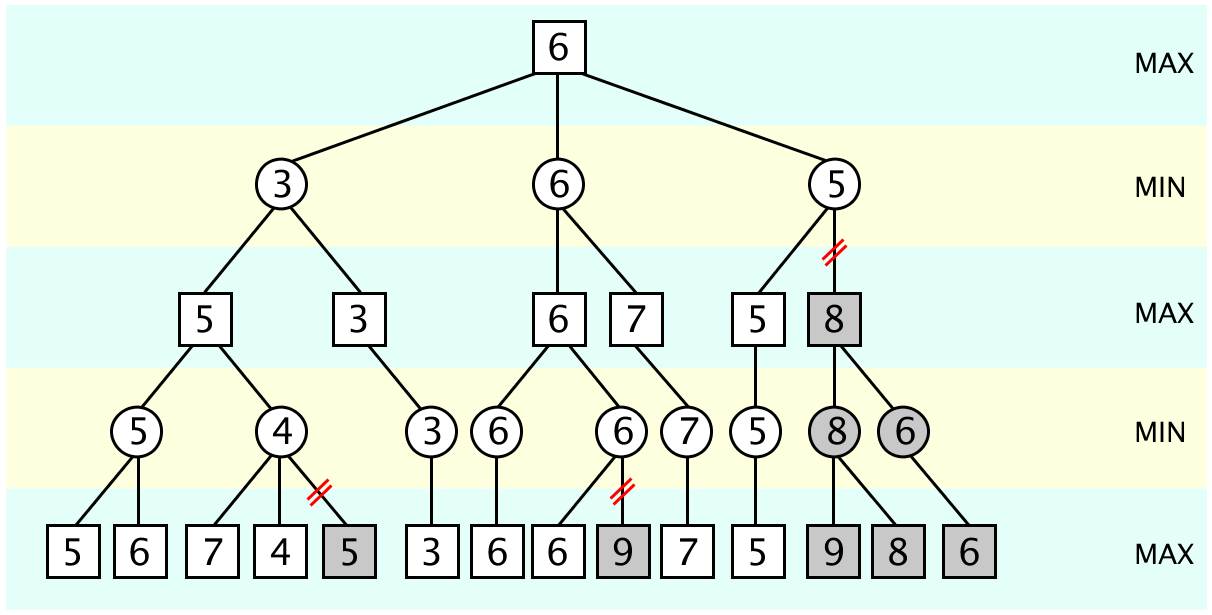
\includegraphics[width=10cm]{alfabeta.png}
 \caption[Algoritem Minimax z alfabeta rezanjem.]{Algoritem minimax z alfabeta rezanjem: slika predstavlja delovanje algoritma minimax z alfabeta rezanjem. Za najblolj desen rez velja: V vozlišču je na potezi igralec MAX in bo vedno izbral vozlišče z maksimalno vrednostjo (trenutno je to vrednost 6). Na nivoju 1 je na potezi igralec MIN in bo vedno izbral minimalno vrednost (v najbolj desnem vozlišču na nivoju 1 je trenutno to 5). Ker pa že vemo, da ima eno izmed vozlišč na nivoju 1 vrednost 6 in ker bo igralec MIN v najbolj desnem vozlišču zagotovo izbral vozlišče z vrednostjo $<=$ 5 (ker imamo 5 že izračunano), lahko na označenem mestu opravimo rez.}
 \label{fig:alfabeta}
\end{figure}

\subsection{Parametri algoritma}
Simulaciji igranja iger je potrebno nastavit nekaj parametrov, ki vplivajo predvsem na hitrost izvajanja in natančnost rezultatov. Eden izmed parametrov je globina minimax drevesa. Globina nam uravnava stopnjo optimalnosti neke poteze, saj z večjo globino drevo razišče večji del prostora. Z večanjem globine, se časovna zahtevnost algoritma eksponentno povečuje. Mi smo se odločili, da bomo uporabljali globino 4

\section{Optimizacija uravnoteženosti}
Za uravnoteževanje bojevnikov smo uporabili genetske algoritme in hill climbing.

\subsection{Genetski algoritmi}
Genetski algoritmi so prilagodljive metode, ki jih uporabljamo za reševanje iskalnih in optimizacijskih problemov. Temeljijo na genetskem procesu bioloških organizmov, saj se zgledujejo po evoluciji v naravi, kjer se populacija neke vrste skozi generacije razvija po načelu naravnega izbora in preživetju uspešnejšega. Genetski algoritmi posnemajo tiste procese v naravi, ki so bistveni za evolucijo. V naravi posamezniki neke populacije med seboj tekmujejo za življenjsko pomembne vire. Hitrejši in pametnejši predstavniki vrste bodo imeli več in boljče vire za preživetje, počasnejši in manj pametni jih bodo dobili težje ali pa sploh ne. Ravno tako se pojavi tekmovanje pri iskanju partnerja za razmnoževanje. Tisti, ki so uspešnejši v preživetju in pri parjenju, bodo po vsej verjetnosti imeli relativno večje število potomcev. Slabši posamezniki jih bodo imeli manj ali pa sploh ne. To pomeni, da se bodo geni dobro prilagojenih oz. ustreznih posameznikov bolj razširili na prihodnje generacije, slabši pa bodo celo izumrli. Kombinacija genov dveh ustreznih staršev
lahko privede do pojava super-ustreznega potomca, ki ima boljše lastnosti od obeh staršev. Na ta način se vrste razvijajo in prilagajajo na svoje okolje.
Ti algoritmi delujejo po analogiji k temu naravnemu procesu. Delujejo nad neko populacijo osebkov (kromosomov), od katerih vsak predstavlja možno rešitev danega problema. Vsakemu kromosomu se priredi ocena uspešnosti, ki je prilagojena iskanemu problemu. Ustreznejši kromosomi - tisti z boljšo oceno - imajo več možnosti za reprodukcijo od ostalih. Nad trenutno populacijo izvedemo simuliran proces evolucije. Iz naše populacije izberemo podmnožico staršev, ki se razmnožujejo. Tako za našo populacijo dobimo nove potomce, ki prevzamejo nekaj lastnosti od vsakega starša. Manj ustrezni predstavniki se bodo razmnoževali z manjšo verjetnostjo in tako izumrli. Na ta način se dobre lastnosti razširijo v naslednje generacije. Če smo genetski algoritem dobro zastavili, bo populacija konvergirala k optimalni rešitvi.
V nadaljevanju bomo predstavili konkretne značilnosti genetskih algoritmov za našo domeno.

\subsubsection{Osnovni pojmi}
\textit{Osebek} je možna rešitev problema. V naši domeni je osebek sestavljen iz dveh bojevnikov, oziroma množice atributov. Osebke imenujemo tudi \textit{kromosomi}.
\\\\
\textit{Geni} so posamezni atributi v osebku.
\\\\
\textit{Kriterijska funkcija} je funkcija, s katero ocenjujemo osebke. Pri nas je ta funkcija definirana kot $\frac{1}{LifeDiff}$, kjer je LifeDiff razlika med življenjema dveh bojevnikov v osebku, kot jo vrne algoritem za simulacijo igre.
\\\\
\textit{Populacija} je množica osebkov. Obdelujemo jo v korakih, ki jih imenujemo \textit{generacija}. Iz osebkov trenutne populacije (\textit{staršev}) tvorimo naslednike (\textit{potomce}), ki pripadajo populaciji naslednje generacije.
\\\\
\textit{Elita} je podmnožica najboljših osebkov v populaciji.
\\\\
\textit{Selekcija}
\\\\
\textit{Križanje}
\\\\
\textit{Mutacija}

\subsection{Hill climbing}



\newpage

%********************************************


\addcontentsline{toc}{chapter}{Seznam slik}
\addtocontents{toc}{\protect\vspace{-2ex}}
\listoffigures

\addcontentsline{toc}{chapter}{Seznam tabel}
\addtocontents{toc}{\protect\vspace{-2ex}}
\listoftables

\newpage





\end{document}

